\section{Regular Expression $\rarr$ Automaton}

\subsection{Thompson method}
Result nondeterministic with $\epsilon$-moves. Map every portion of the r.e. to a piece of the automaton. Every piece of the automaton must have a unique and final state.

\begin{figure}[H]
    \centering
    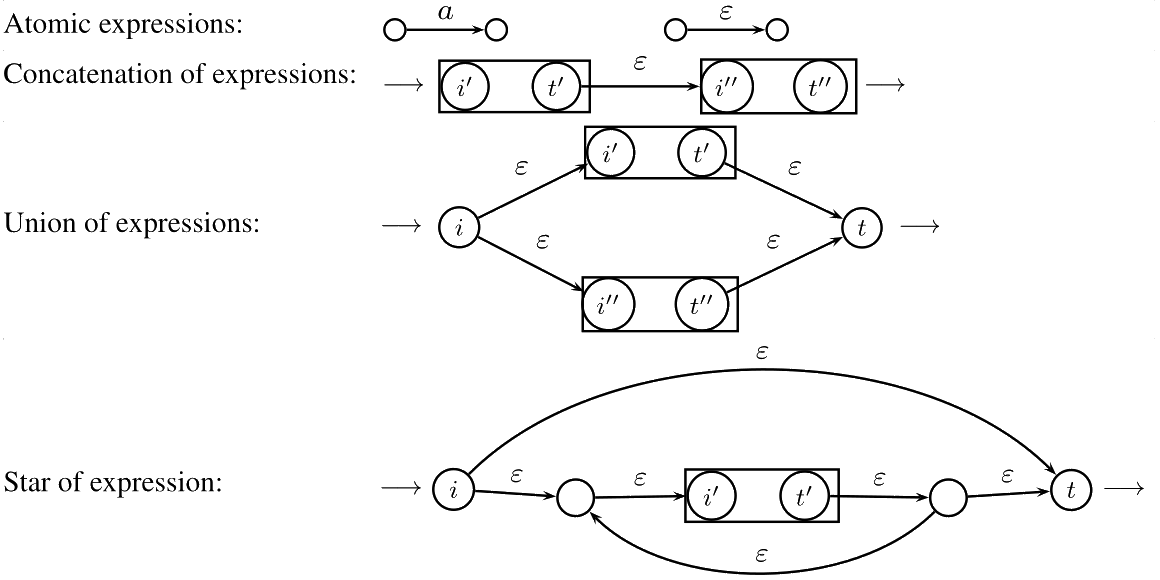
\includegraphics[width=\linewidth]{automata/thompson.png}
\end{figure}

\subsection{Berry-Sethy method}

Result deterministic but can be non-minimal.

\subsubsection{Locally Testable Languages (LOC)}

Proper subfamily of REG. Assuming $a,b \in \Sigma$, $x, y \in \Sigma^*$, define $Ini(L) = \{a | ax \in L\}$, $Fin(L) = \{b | xb \in L\}$, $Dig(L) = \{ab | xaby \in L\}$.

\begin{align*}
    L \in \text{LOC} &\iff \\
    L \setminus \{\epsilon\} = \{&x | Ini(x) \in Ini(L) \land \\
    &Dig(x) \subseteq Dig(L) \land \\
    &Fin(x) \in Fin(L) \}
\end{align*}

To prove that a language is not local provide a string $x\notin L$ s.t. $Ini(x) \in Ini(L) \land Dig(x) \subseteq Dig(L) \land Fin(x) \in Fin(L)$.

\subsubsection{Recognizer for Local Languages}

A unique initial state $q_0$, a state for each terminal, the finals are the $Fin$. If $\epsilon \in L$ then also $q_0$ is final. $q_0$ is connected to the $Ini$, and the states are connected if the pair is in $Dig$.

\subsubsection{Berry-Sethi method}

Given $e$ the initial r.e., $e'$ is the numbered version over alphabet $\Sigma_N$. Conside expression $e' \dashv$. Define for each symbol $a$ of $e'$ the set $Fol(a) = \{b | ab \in Dig(e'\dashv)\}$.

Every state is a subset of $\Sigma_N \cup \{\dashv\}$, containing all the symbols that may follow in the input. The initial state contains $Ini(e'\dashv)$. The states are generated adding transitions until a fixed point is reached. The final states are the ones containing $\dashv$.

\begin{algorithm*}[H]
    \caption{Berry-Sethi}
    \SetAlgoLined
    $q_0 = Ini(e'\dashv)$;
    $Q = \{q_0\}$;
    $\delta=\emptyset$\;
    \While{$\exists q \in Q$ not visited}{
        mark $q$ as visited\;
        \For{$b \in \Sigma$}{
            $q' = \cup_{\forall b_i \in q} Fol(b_i)$\;
            \If{$q' \notin Q$}{
                mark $q'$ as not visited\;
                $Q = Q \cup \{q'\}$
            }
            $\delta = \delta \cup \{q \xrightarrow{b} q'\}$
        }
    }
\end{algorithm*}
